% vim:ft=tex
% rubber: module xelatex
\section{Our program}
\label{sec:prog}
Our program is written in C++ using the Qt and OpenCV libraries. The application
consists of a Qt-based GUI that allows the user to load images, select between
various image processors, select parameters and peruse the results of the
processing by zooming and panning on the output image. Furthermore, it is
possible to select points of interest (POIs) by double clicking on the image,
which can be used to select points for the calibration algorithm. The GUI also
has a log output window for textual output from the algorithms. It is possible
to perform every step of functional face recognition, from the calibration that
provides the rectification data to the final PCA analysis, within the system we
have built.

Each processor is implemented as a class that specifies which parameters are
available to it. The parameters can be set by the user with the help of the Qt
property system and the QPropertyEditor library. After parameterisation, the
actual processing is performed in a separate thread, keeping the interface
responsive and making it possible for the user to cancel a long-running
processor.

% vim:ft=tex
% rubber: module xelatex
\subsection{Rectification}
\label{sec:rectification}

We have implemented image rectification based on our previous work in camera calibration.
We use the intrinsic and extrinsic parameters calculated by the calibration to
construct the specific perspective transformation that is required to rectify a pair of stereo images.

We obtain the following values from the calibration:
\begin{itemize}
\item $T_l, T_r$, translation vectors from the calibration object to the left
  and right camera origins respectively, in the camera reference frames.
\item $R_l, R_r$, rotation matrices from the calibration object reference system to
  the left and right camera reference systems respectively.
\item $f_l, f_r$, the focal lengths of the left and right cameras.
\end{itemize}

These parameters allow us to compute the following values:
\begin{itemize}
\item $R=R_lR_r^{-1}$, the rotation matrix from the right to the left reference
  frame.
\item $T=RT_r$-$T_l$, the translation vector from the left to the right camera
  origin, in the left camera reference frame.
\item $R_{rect}$, the rectification rotation matrix. This is computed by
  creating an orthonormal base where $X$ is the translation vector $T$, $Y$ is the cross
  product of the unit vector with $X$ (in the $Z$-axis direction), and $Z$ is the
  cross product of $X$ and $Y$.\footnote{ All vectors are normalised to unit length.}
\item $f$, the mean of the left and right focal lengths.
\end{itemize}

The rectification process then proceeds as follows. Using these values, the left image is
rectified by $R_{rect}$, and the right image is rectified by $RR_{rect}$. The
rectification coordinates are computed in 3D space, by casting the pixel
coordinates into three-dimensional coordinates, offset so that (0,0) is the
middle of the image. The $z$ component of these coordinates is the focal length. The rectification matrices are then applied to these new coordinates to get the rectified pixel coordinates.

The values are multiplied by $\frac{f}{z}$, returning the $z$ values of the new coordinates to the focal length. We use OpenCV \texttt{remap()} function to perform the actual remapping of pixels and to
interpolate non-existent pixels. Bicubic interpolation in a $4\times4$ pixel neighbourhood
is used for this last step.

\subsubsection{Testing rectification accuracy}
To test the accuracy of the rectification, we took six images with a chessboard pattern on them and rectified them. We used the OpenCV algorithm for extracting grid corners of a chessboard on the rectified images, acquiring a list of pixel positions for the corners in the image.

We then compared the $y$ coordinates of these pixels. In an accurate rectification, all the chessboard corners on a line would appear in the same scanline in the rectified image, and therefore should have the same $y$ coordinates. The disparities between $y$ coordinates can therefore be used as a measure of rectification error.

The mean errors for the six images we tested are listed in
table~\ref{tab:rectification-error}. Each image has 80 interior chessboard corners, and the image mean values are across all these corners. The overall
mean and standard deviation are also given, as the mean for all six images (i.e.
480 corners). The accuracy of the results show that overall, there is room for improvement, but they are not completely unreasonable. Our initial experiments showed that
the quality of the calibration data has a very large impact on the accuracy of the
rectification; the errors given here are for the best calibration data we were
able to obtain from the test images. A more accurate calibration could improve our rectification results considerably.

\begin{table}[h]
  \centering
  \begin{tabular}{c c c}
    \toprule
    Image & Mean error & Std dev \\
    \midrule
    DSCF4060 & 3.57  & 1.70 \\
    DSCF4061 & 3.68  & 1.60 \\
    DSCF4062 & 7.01  & 1.67 \\
    DSCF4063 & 4.40  & 1.81 \\
    DSCF4065 & 7.75  & 1.41 \\
    DSCF4066 & 7.16  & 1.84 \\
    \midrule
    Average  & 5.60  & 1.67 \\
    \bottomrule
  \end{tabular}
  \caption[Rectification errors]{Rectification errors. This table gives the mean error and
    standard deviation for the vertical displacement between the same points
    between the left and right images. These points are 80 grid corners extracted from chessboard images.}
  \label{tab:rectification-error}
\end{table}


% vim:ft=tex
% rubber: module xelatex

\subsection{Stereo matching}
\label{sec:stereo}
We have implemented dynamic programming based stereo matching using the methods
described by \citet{realtimestereo}. The output of the stereo matching is a
disparity map for each of the left and right images; the disparity map is a grey
scale image with black (or 0) signifying the lowest disparity, and white (or
255) signifying the maximum disparity. The disparity map is built using a
dynamic programming matrix for each scan line in the image; in the simplest
case, the process is as follows (for each scan line):

\begin{enumerate}
\item Create the dynamic programming matrix, $A$, with width and height both
  equal to the length of the scan line (i.e. the width of the images).
  Initialise the top-left corner to 0.

\item Step through the matrix, calculating $A[i,j] = \mathrm{min}(A[i-1,j],
  A[i,j-1], A[i-1,j-1]) + \mathrm{diff}(\mathrm{imageL}[i], \mathrm{imageR}[j])$
  where \texttt{diff} gets the difference between the image pixel values in the
  current scan line.

\item Calculate the path of minimal cost through the matrix $A$, starting in the
  bottom right corner, and moving from there to the adjacent position with the
  minimum value, i.e. $\mathrm{min}(A[i-1,j], A[i,j-1], A[i-1,j-1])$. Fill the
  disparity map with the appropriate value ($\mathrm{DisparityMapL}[i,y]=j-i$,
  $\mathrm{DisparityMapR}[j,y]=i-j$).
\end{enumerate}

After having built up the disparity maps for the entire image (i.e. after doing
the above for all scan lines), go through them and normalise the values to the
range $[0,255]$, or, alternatively multiply the matrices by a user configurable
factor.

In addition to the simple version of the disparity mapping algorithm described
above, we have implemented the following (optional) modifications, in order to
improve the quality of the matching:

\begin{enumerate}
\item It is possible to assign an additional bonus or penalty to moving
  diagonally in the dynamic programming matrix, depending on whether we want
  smooth or spiky (very disparate) images respectively.

\item The choices for each scan line can be modified by those for the previous
  scan line, reducing error by ``suggesting'' ways to conform.

\item A median filter can be applied to the stereo images before building the
  disparity map, to get rid of noise.

\item It is possible to go through the dynamic programming matrix not only from
  the bottom-right to top-left corner, but also from top-left to bottom-right,
  and then choose the least-weight path overall. This helps reduce the cases
  where one of them goes horribly off the 'best' path because it, intuitively,
  followed the lowest-weight path into a dead end.

\item The running time can be improved by selecting a maximum disparity bound,
  $b$. The ``path of least resistance'' is never allowed to go outside this
  disparity bound because we set $A[i,j]$ to a vast positive value if $i > b$ or
  $j > b$.
\end{enumerate}


%%% Leaving this out for now...
% One improvement we didn't implement: line skipping. (In that version, at
% thebeginning, every n’th horizontal line is calculated to find bounding space
% for possible disparities in between.)


\subsubsection{Testing of stereo matching}

\begin{figure}[p]
  \centering
  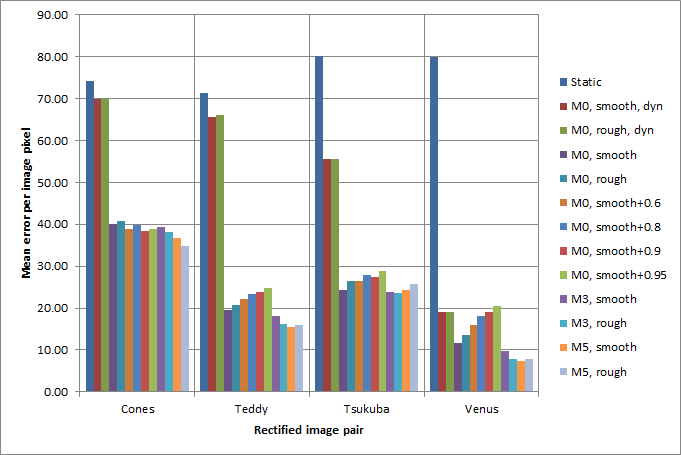
\includegraphics[height=0.4\textheight]{Stereo-left-report}\\[2mm]
  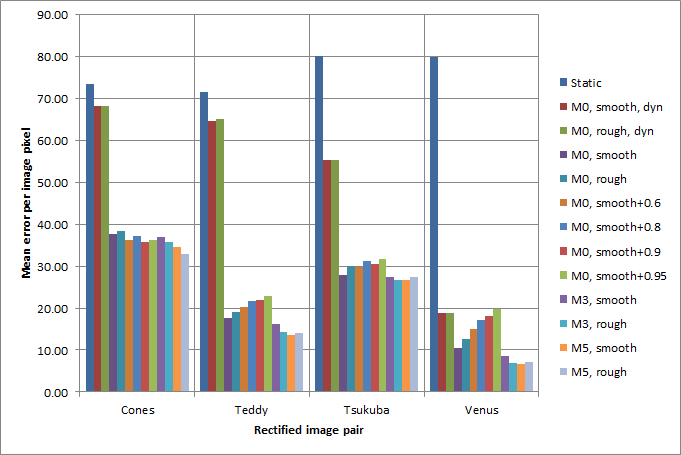
\includegraphics[height=0.4\textheight]{Stereo-right-report}
  \caption[Results of stereo matching]{Results of stereo matching for the left
    (top graph) and right (bottom graph) images, using various parameters.
    Resulting depth maps are compared to the canonical depth maps to obtain
    discrepancies (quantities of error). Each coloured column in the chart is a
    different parameterisation, as tested on one of the four images. `Static' is
    the baseline difference between the canonical depth map and a image with
    randomised values. `M0' indicates a median filter was not used in
    preprocessing. `M3' and `M5' indicate median filters of size 3 and 5
    respectively. `rough' indicates scanlines did not influence each other.
    `smooth' indicates each scanline was influenced by the one previous, by 0.5
    by default or by the amount given. `dyn' indicates the depth map was created
    by stretching the disparities to the full [0...255] range, instead of
    multiplying by the value recommended by \cite{middlebury} for each
    particular image.}
  \label{fig:stereo-report}
\end{figure}

We took the best results and submitted them to the Middlebury online tests.
\cite{stereocorrespondence, middlebury} Their calculator unfortunately
presupposes a cyclopean image, which we were not calculating. We submitted left
and right instead, and chose the better of the two in each case. Still, we
expect we would have scored considerably higher if we had calculated the
cyclopean images. However, the details of our implementation made this
difficult.

We had 44.9\% to 45.8\% bad pixels total. The worst Middlebury have on record is
20.7\%. \cite{stereocorrespondence, middlebury} For our test disparity maps,
`Tsukuba' was best with 17.9\% error. `Venus' and `Teddy' were mediocre with
40.5\% and 54.4\% respectively. `Cones' was worst with 69.0\%. See
figure~\ref{fig:stereo-report} for full details.

\begin{figure}[p]
 \centering

 \subfloat[Tsukuba (rough)] { \label{fig:tsu-1} 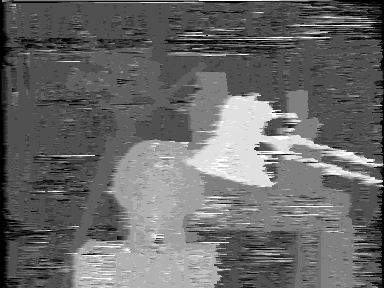
\includegraphics[trim = -2mm -2mm -2mm -2mm, width=0.23\textwidth]{stereo/tsu_imL_mat0_hardmult} }
 \subfloat[Venus (rough)] { \label{fig:ven-1} 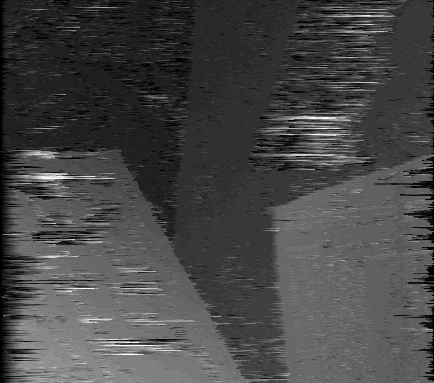
\includegraphics[trim = -2mm -2mm -2mm -2mm, width=0.23\textwidth]{stereo/ven_imL_mat0_hardmult} }
 \subfloat[Cones (rough)] { \label{fig:con-1} 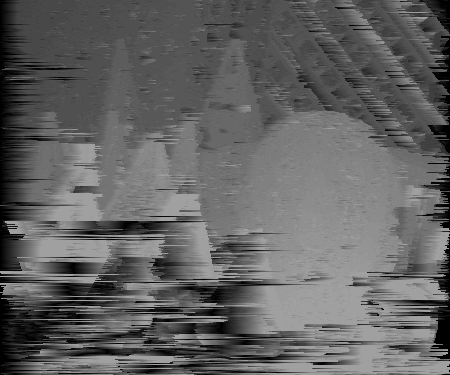
\includegraphics[trim = -2mm -2mm -2mm -2mm, width=0.23\textwidth]{stereo/con_imL_mat0_hardmult} }
 \subfloat[Teddy (rough)] { \label{fig:ted-1} 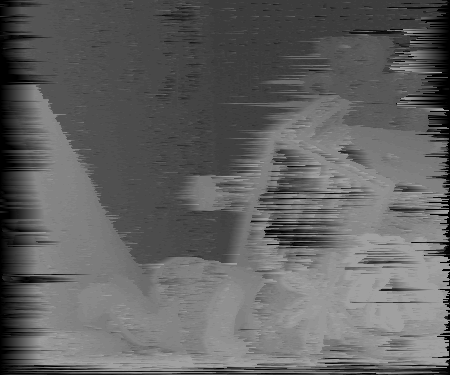
\includegraphics[trim = -2mm -2mm -2mm -2mm, width=0.23\textwidth]{stereo/ted_imL_mat0_hardmult} }\\

 \subfloat[Tsukuba (mid)] { \label{fig:tsu-2} 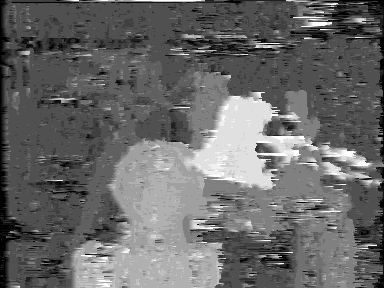
\includegraphics[trim = -2mm -2mm -2mm -2mm, width=0.23\textwidth]{stereo/tsu_imL_mat5_hardmult_smooth} }
 \subfloat[Venus (mid)] { \label{fig:ven-2} 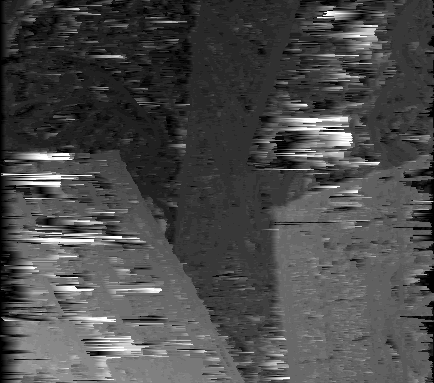
\includegraphics[trim = -2mm -2mm -2mm -2mm, width=0.23\textwidth]{stereo/ven_imL_mat5_hardmult_smooth} }
 \subfloat[Cones (mid)] { \label{fig:con-2} 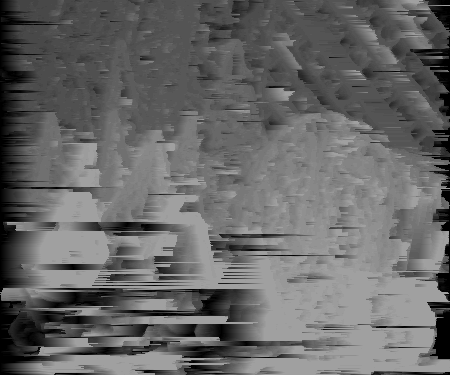
\includegraphics[trim = -2mm -2mm -2mm -2mm, width=0.23\textwidth]{stereo/con_imL_mat5_hardmult_smooth} }
 \subfloat[Teddy (mid)] { \label{fig:ted-2} 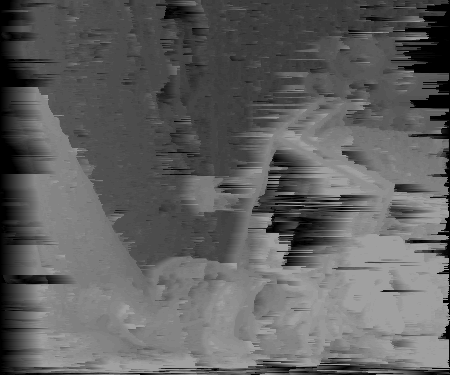
\includegraphics[trim = -2mm -2mm -2mm -2mm, width=0.23\textwidth]{stereo/ted_imL_mat5_hardmult_smooth} }\\

 \subfloat[Tsukuba (smooth)] { \label{fig:tsu-4} 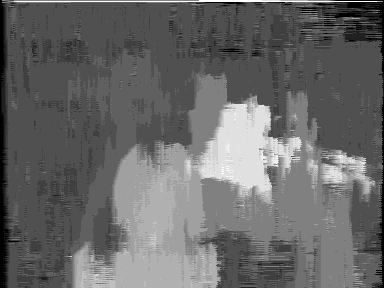
\includegraphics[trim = -2mm -2mm -2mm -2mm, width=0.23\textwidth]{stereo/tsu_imL_mat0_hardmult_smooth0.9.png} }
 \subfloat[Venus (smooth)] { \label{fig:ven-4} 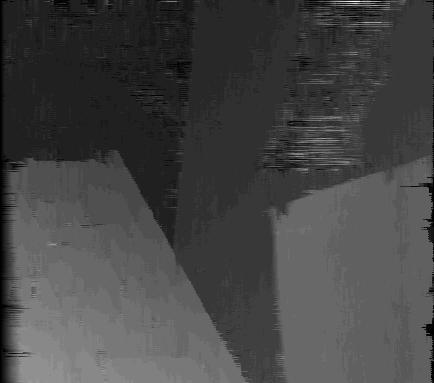
\includegraphics[trim = -2mm -2mm -2mm -2mm, width=0.23\textwidth]{stereo/ven_imL_mat0_hardmult_smooth0.9.png} }
 \subfloat[Cones (smooth)] { \label{fig:con-4} 
\includegraphics[trim = -2mm -2mm -2mm -2mm, width=0.23\textwidth]{stereo/con_imL_mat0_hardmult_smooth0.9.png} }
 \subfloat[Teddy (smooth)] { \label{fig:ted-4} 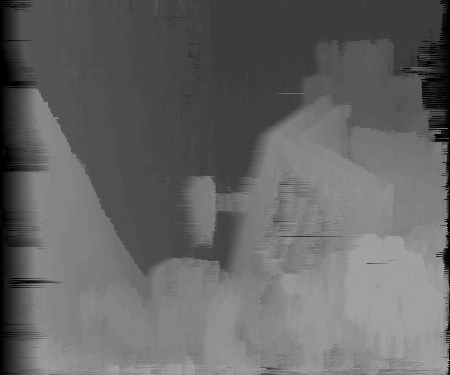
\includegraphics[trim = -2mm -2mm -2mm -2mm, width=0.23\textwidth]{stereo/ted_imL_mat0_hardmult_smooth0.9.png} }

 \subfloat[Tsukuba (ideal)] { \label{fig:tsu-i} 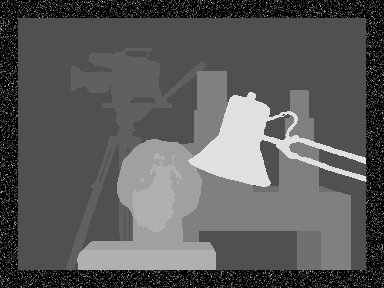
\includegraphics[trim = -2mm -2mm -2mm -2mm, width=0.23\textwidth]{stereo/tsu_ideal_L} }
 \subfloat[Venus (ideal)] { \label{fig:ven-i} 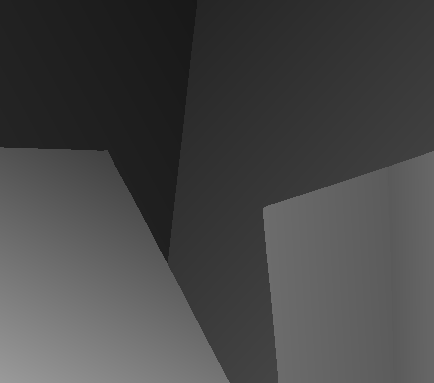
\includegraphics[trim = -2mm -2mm -2mm -2mm, width=0.23\textwidth]{stereo/ven_ideal_L} }
 \subfloat[Cones (ideal)] { \label{fig:con-i} 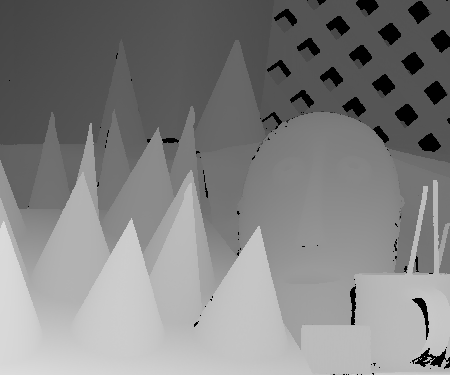
\includegraphics[trim = -2mm -2mm -2mm -2mm, width=0.23\textwidth]{stereo/con_ideal_L} }
 \subfloat[Teddy (ideal)] { \label{fig:ted-i} 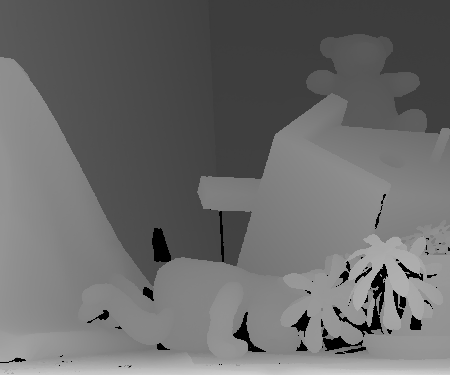
\includegraphics[trim = -2mm -2mm -2mm -2mm, width=0.23\textwidth]{stereo/ted_ideal_L} }\\

 \caption[Examples of dynamic programming with various parameters]{Examples of
   dynamic programming with various parameters. Canonical baseline images are
   courtesy of \citet{stereocorrespondence}. `rough' images are not
   preprocessed. `mid' images have a 5x5 median filter applied in preprocessing
   and feature inter-scanline smoothing with a weight of 0.5. `smooth' images
   feature inter-scanline smoothing with a weight of 0.9.}
 \label{fig:stereo-image-depth-maps}
\end{figure}

\begin{figure}[p]
 \centering
 \subfloat[Depth map (no smoothing)] { \label{fig:sm-1} 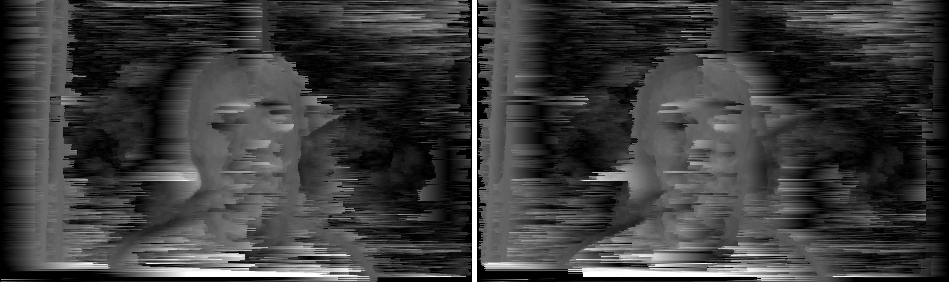
\includegraphics[trim = -2mm -2mm -2mm -2mm, width=0.8\textwidth]{stereo/lowsmooth} }\\
 \subfloat[Depth map (low smoothing)] { \label{fig:sm-2} 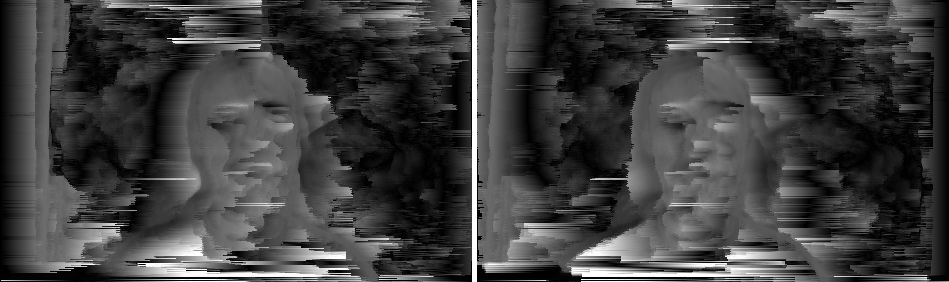
\includegraphics[trim = -2mm -2mm -2mm -2mm, width=0.8\textwidth]{stereo/midsmooth} }\\
 \subfloat[Depth map (mid smoothing)] { \label{fig:sm-3} 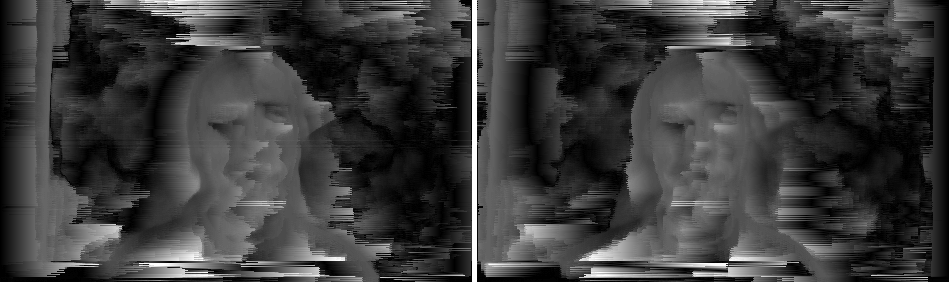
\includegraphics[trim = -2mm -2mm -2mm -2mm, width=0.8\textwidth]{stereo/highsmooth} }\\
 \subfloat[Depth map (high smoothing)] { \label{fig:sm-4} 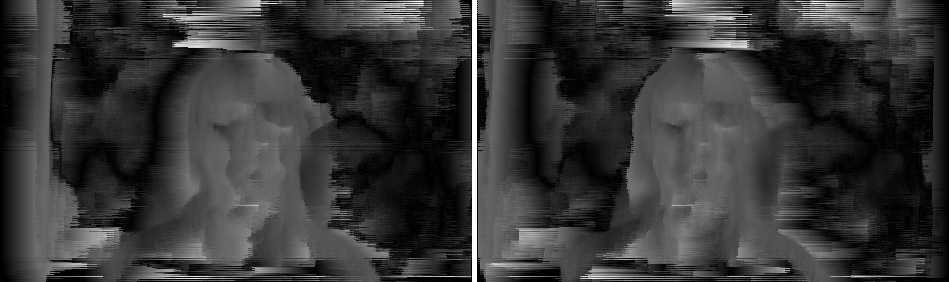
\includegraphics[trim = -2mm -2mm -2mm -2mm, width=0.8\textwidth]{stereo/extremesmooth} }
 \caption[Depth maps for stereo pairs created with various parameters]{Depth
   maps for one of the stereo pairs in our database, calculated using increasing
   levels of smoothness.}
 \label{fig:stereo-pair-depth-maps}
\end{figure}

Consider Figure~\ref{fig:stereo-pair-depth-maps}. Increasing the three
smoothness parameters - median matrix size, inter-scanline smoothing, and
diagonal preference / disparity penalty - often results in less noise, but loss
of definition.

% vim:ft=tex
% rubber: module xelatex

\subsection{Face recognition}
\label{sec:face-rec}
We have implemented face recognition based on PCA analysis of the image pixel
values (the holistic approach). Face recognition is effectively the culmination of all our work so far.

Our first step is to preprocess the image database. Images must first be rectified (see section~\ref{sec:rectification}). Preprocessing ensures that a fixed triple of face features (the outer corners of the eyes, and the point between the base of the nose and the lip) are in the same positions for all images. For further details, see section~\ref{sec:preprocess} below. PCA is performed on these processed images.

Up to six channels of data from each image can be used: values for red, green and blue, values for hue and saturation, and depth values. Depth values are created by running our stereo matching algorithm (see section~\ref{sec:stereo}) on the preprocessed images to create equivalent-sized depth maps.\footnote{ It is important at this step to use a fixed multiplier for disparities in all the images, rather than dynamically calculating how to best map the disparities in an image to [0...255]. This is so that representations of relative distances are fixed across all images in the dataset.}

For each pixel in the image in turn, the $n$ data points are concatenated into a series of values, and appended to the single column image vector. The result is a single vector of length $L = n \times m$, where $m$ is the total number of pixels in the image.

For the training phase of the PCA processing, the average image vector for the
training set is computed, and subtracted from each image vector to create the normalised vectors. Each vector is multiplied by its inverse, and the resulting matrices are summed to acquire the overall covariance matrix. This matrix essentially holds all the information of the database of images.

The next step requires that the eigenvectors and eigenvalues of the matrix be calculated. Because the size of the matrix is $L^{2}$, this is computationally expensive. We were able to achieve reduction of dimensionality by using the OpenCV PCA library functions in our code. OpenCV implements the variation introduced by \citet{turk_pentland}, whereby the eigenvectors and eigenvalues are calculated by a square matrix whose dimensionality is equal to the the number of images in the database - a considerable reduction. This allows us to achieve training and matching in a reasonable time and with reasonable memory consumption.

The highest eigenvalues represent those components (`directions') for which we have the greatest variance, i.e. discriminating power. The eigenvectors associated with those highest eigenvalues are kept. The number to keep is a user-configurable parameter. The program calculates the fractional quantity $Q$ of face information being stored by dividing the sum of the \emph{kept} eigenvalues by the sum of \emph{all} the eigenvalues. The user can therefore trade off efficiency (in terms of memory and time) against quality by choosing to keep a number of components such that $Q \geq t$ for some threshold $t$.

The result is a set of eigenvectors which give us an orthonormal basis, or higher-dimensional `principal component space'. Each training image is projected into this space, and for each class of images (i.e. each person whose image was taken), the \emph{average image vector} (in the principal component space) is computed. The maximum distance between
the average image and the set of original training images for that class is also calculated. This maximum distance
(multiplied by some user-configurable factor) is used as a cutoff distance when
matching; images that do not match any classes within the cutoff distance are
considered a no-match.

The program uses this same metric to gauge the confidence in a prediction. Images which, when projected into the orthonormal basis, are close to the edge of the `point cloud' of training examples for the closest-fitting class, are less likely to have been \emph{correctly} matched to that class than those very near to the average image vector.

To test the accuracy of the classification, each training image is projected
into the eigenspace and back; the error between the original image and the
reconstructed image (as the square of the distance) is calculated. Sample results for
this are shown in section~\ref{sec:pcaresults} below.

When given an image to classify, matching is performed as follows. The image vector is constructed as for the training set, using $n$ channels and resulting in a vector length $n \times image_height \times image_width$. The overall average vector is subtracted, and the vector is projected into the PCA space. The distance of this projection to each class average vector is computed. The class vector that is nearest to the test image is considered a match if it is closer than the cutoff depth for that class. Our program by default returns the closest match and the next-closest match, stating the confidence in each guess.

\subsubsection{Preprocessing of images}
\label{sec:preprocess}

Before doing PCA analysis on the face images, they are preprocessed or `registered' to make sure
face features are in (almost) the same positions on all the images. Initially, we operate on rectified images, i.e. stereo images that have
been projected into a geometry in which they have corresponding horizontal epipolar lines. The
rectification step helps diminish unwanted deformation caused by the later steps of the
preprocessing, and also prepares the images for stereo mapping if we wish to use depth data for PCA.

After rectification, face features are manually identified. The features
identified are the outer corners of the eyes, and the point above the lip on the vertical centre of the nose 
(since these features are fairly definable, and seem to be in approximately the same position regardless
of facial expression). For each of these feature points $p$, the average $p'$of each feature point over the whole image
training database is found. Each image is geometrically transformed so that its three feature points align to the location of $p'$.

This is done by solving (for each image) the affine transformation needed to transform the feature point
locations for that image into the average location $p'$, using singular value
decomposition of the resulting set of matrices. This is applied as an affine
transformation to the whole image. Pixel interpolation is performed to create the new image. All three steps are done using OpenCV functions.

Following the transformation, the images are cropped to a user-configurable
ratio. The ratio is determined by adding some factor of the vertical and horizontal distances
between the feature points to the edges of the image. An ellipse is then fitted to the boundaries of the cropped image. Everything outside this ellipse is
`blacked out' to zero values. Finally, the image is scaled down to a fixed width (also
user-configurable), to speed up the processing.

Finally, we apply our stereo matching implementation to the processed images to
yield the depth map that can optionally be used in the PCA matching. The last channels - Hue and Saturation values - are extracted from each pixel by a function during the processing.

\subsubsection{Testing face recognition}
\label{sec:pcaresults}

Methodology: for each test, use whatever number of components means keeping at least 80\% image information (in terms of fraction of the total eigenvalues). Set error threshold to a relatively strict $1.0$, i.e. only identify test images as belonging to a class if the variation between them and the class mean is less than or equal to the maximum variation within the training images for that class. Use half our face database of 88 images to train, and half to test. There are 11 classes in the database.

Consider Table~\ref{tbl:face-rec-1}. The amount of image information being retained when a certain number of components are kept is not heavily dependent on the image size. There is little difference between sizes. In all cases, 12 or 13 components are required for the 80\% information threshold we use in our other experiments.

\begin{table}[h!]
  \centering
  \begin{tabular}{c c c c c}
    \toprule
    \textbf{ } & \textbf{} & \textbf{Image size} & \textbf{} & \textbf{}\\
    \textbf{ } & \textbf{ 32x49 } & \textbf{ 64x99 } & \textbf{128x198} & \textbf{256x396}\\
    \midrule
    \textbf{2 components} & 39.6\% & 39.9\% & 38.8\% & 37.8\% \\
    \textbf{4 components} & 55.6\% & 56.0\% & 55.5\% & 53.2\% \\
    \textbf{6 components} & 64.8\% & 65.2\% & 64.0\% & 62.2\% \\
    \textbf{8 components} & 71.9\% & 72.4\% & 70.5\% & 69.3\% \\
    \textbf{10 components} & 77.2\% & 77.6\% & 76.1\% & 74.6\% \\
    \textbf{12 components} & 80.8\% & 81.3\% & 79.8\% & 78.4\% \\
    \textbf{14 components} & 83.8\% & 84.4\% & 82.3\% & 81.6\% \\
    \textbf{16 components} & 86.3\% & 86.8\% & 85.7\% & 84.2\% \\
    \bottomrule
  \end{tabular}
  \caption[Information retained in face recognition tests for different-sized images]{Information retained in face recognition tests for different-sized images. Each row is a case where a different number of components were kept. Each column is a different image dimensionality. Results are presented as percentage of total summed eigenvalues. In each case, PCA was performed on all six possible channels, on a training set of 44 images with 11 classes.}
  \label{tbl:face-rec-1}
\end{table}

Consider Table~\ref{tbl:face-rec-2}. As expected, we have better reconstruction when we keep more principal components. The total improvement when we go from 4 components to 10 is 41695. The total improvement when we go from 10 components to 16 is 12489. This apparent diminishing returns is because we start including more `important' (in terms of their associated eigenvalue) eigenvectors, and then start adding ones which lend less to the PCA.

\begin{table}[h!]
  \centering
  \begin{tabular}{c c c c}
    \toprule
    \textbf{ } & \textbf{4 components} & \textbf{10 components} & \textbf{16 components} \\
    \textbf{ } & \textbf{(53.2\% image data retained)} & \textbf{(74.6\% image data retained)} & \textbf{(84.2\% image data retained)} \\
    \midrule
    \textbf{Class A} & 9848 & 9018 & 6670\\
    \textbf{Class B} & 11238 & 7853 & 6170\\ 
    \textbf{Class C} & 11719 & 7811 & 7376\\ 
    \textbf{Class D} & 12061 & 7736 & 6560\\
    \textbf{Class E} & 10268 & 7873 & 6383\\
    \textbf{Class F} & 13339 & 8683 & 7001\\ 
    \textbf{Class G} & 10252 & 9022 & 6516\\ 
    \textbf{Class H} & 14167 & 7331 & 5709\\
    \textbf{Class I} & 11945 & 10223 & 7379\\
    \textbf{Class J} & 11196 & 9187 & 6075\\ 
    \textbf{Class K} & 11586 & 8267 & 7596\\
    \bottomrule
  \end{tabular}
  \caption[Sample reconstruction error for the 256x396 size images]{Sample reconstruction error for the 256x396 size images, with PCA performed on all six possible channels. A training set of 44 images with 11 classes was used. Each column is the error for one class (person) in the training set. Error is measured in absolute difference between the original training example image vector and the reconstructed vector projected back out of the PCA space. Each row is a case where a different number of components were kept, with the quantity of information retained (as a percentage of total summed eigenvalues) in brackets.}
  \label{tbl:face-rec-2}
\end{table}

Consider Table~\ref{tbl:face-rec-3}. Note that most often, PCA failed on the classes or test images for the person whose hand was over his face, the person who had the most different positions and expressions, the person who had only two training images, or the person wearing a hat. These are classes F, C, H, K respectively in Table~\ref{tbl:face-rec-2}. Very few test images outside of these unexpected cases were misclassified or unclassified. Note that classes F and H have the highest reconstruction error when only a few components are kept: PCA is unable to reconstruct the considerable variance \emph{within} the class at a lower dimensionality.

In general, though, we observe that those classes of images with the greatest variance in pose, lighting or expression are \emph{not necessarily} the hardest to classify. It simply means that we have less confidence when we classify into that class. These highly varying images did, however, result in a broad `point cloud' in higher-dimensional PCA space, so when any test image was misclassified, it had a greater-than-average chance to be misclassified into a highly varying class.

\begin{table}[h!]
  \centering
  \begin{tabular}{c c c c c}
    \toprule
    \textbf{ } & \textbf{} & \textbf{Image size} & \textbf{} & \textbf{}\\
    \textbf{ } & \textbf{ 32x49 } & \textbf{ 64x99 } & \textbf{128x198} & \textbf{256x396}\\
    \midrule
    \textbf{Number} & {} & {} & {} & {} \\
    \textbf{successfully} & 30 & 32 & 33 & 34\\
    \textbf{classified} & {} & {} & {} & {} \\
    \midrule
    \textbf{Number} & {} & {} & {} & {} \\
    \textbf{failed to} & 14 & 9 & 7 & 4\\
    \textbf{classify} & {} & {} & {} & {} \\
    \midrule
    \textbf{Number} & {} & {} & {} & {} \\
    \textbf{partially} & 0 & 2 & 3 & 4\\
    \textbf{misclassified} & {} & {} & {} & {} \\
    \midrule
    \textbf{Number} & {} & {} & {} & {} \\
    \textbf{completely} & 0 & 1 & 1 & 2\\
    \textbf{misclassified} & {} & {} & {} & {} \\
    \bottomrule
  \end{tabular}
  \caption[Results of classification testing for different-sized images]{Results of using PCA for face recognition of new images (classification testing). Four different image sizes are tested. A training set of 44 images with 11 classes was used, and in all cases, PCA was performed on all six possible channels. A number of principal components sufficient to retain 80\% image data were used. Each column is a different image dimensionality. `Number successfully classified' is the number of test images correctly classified. `Number failed to classify' is the number of test images the processor was not confident enough to enter a guess for. `Number partially misclassified' is the number of test images for which the processor's second guess was correct. `Number completely misclassified' is the number of test images for which the processor's initial and secondary guesses were both incorrect.}
  \label{tbl:face-rec-3}
\end{table}

Note in Table~\ref{tbl:face-rec-3} that as we increase image size, we see better classification, and also transference of complete failures to classify into misclassifications. By the biggest size, more images are misclassified than unable to classify.

\begin{table}[h!]
  \centering
  \begin{tabular}{c c c c c}
    \toprule
    \textbf{ } & \textbf{ RGB } & \textbf{ RGB + HS } & \textbf{RGB + Depth} & \textbf{RGB + HS + Depth}\\
    \midrule
    \textbf{Number} & {} & {} & {} & {} \\
    \textbf{successfully} & 29 & 34 & 31 & 34\\
    \textbf{classified} & {} & {} & {} & {} \\
    \midrule
    \textbf{Number} & {} & {} & {} & {} \\
    \textbf{failed to} & 7 & 5 & 6 & 4\\
    \textbf{classify} & {} & {} & {} & {} \\
    \midrule
    \textbf{Number} & {} & {} & {} & {} \\
    \textbf{partially} & 5 & 4 & 5 & 4\\
    \textbf{misclassified} & {} & {} & {} & {} \\
    \midrule
    \textbf{Number} & {} & {} & {} & {} \\
    \textbf{completely} & 3 & 1 & 2 & 2\\
    \textbf{misclassified} & {} & {} & {} & {} \\
    \bottomrule
  \end{tabular}
  \caption[Results of classification testing for different numbers of channels]{Results of using PCA for face recognition of new images (classification testing), using different channels. RGB, HSV and depth map data are tested. Each column specifies a different combination. A training set of 44 images, of dimension 256x396, with 11 classes was used. `Number successfully classified' is the number of test images correctly classified. `Number failed to classify' is the number of test images the processor was not confident enough to enter a guess for. `Number partially misclassified' is the number of test images for which the processor's second guess was correct. `Number completely misclassified' is the number of test images for which the processor's initial and secondary guesses were both incorrect.}
  \label{tbl:face-rec-4}
\end{table}

Table~\ref{tbl:face-rec-4} shows the results of using different channels. In general, the more tracked data, the better. PCA generally worked well even with simple RGB data. While we cannot say so with statistical rigour, it does appear that the Hue and Saturation values may be more useful than the depth data. This may be because those disparity maps were created by stereo matching on \emph{preprocessed} images: the images began as rectified stereo pairs, but underwent an affine transformation before stereo matching. This means the depth map quality was noticeably lower than usual.

The beauty of the PCA process is that even if we were using random noise for depth maps, it would not matter: PCA will simply learn that those data values are not good discriminators (and therefore predictors); any eigenvector along the `direction(s)' of depth would not have a high eigenvalue, and therefore would not be chosen as a principal component.

These observations are only valid given our particular (relatively strict) cutoff point or `confidence tolerance' for classification. Some data channels might have proven themselves better or worse if we had required the system to return a guess for the class of every single test image, including those that are hard to classify.

\begin{figure}[h]
 \centering

 \subfloat { \label{fig:row1-1} 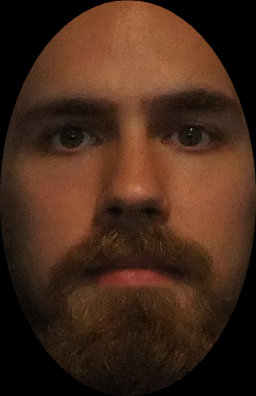
\includegraphics[trim = -1mm -1mm -1mm -1mm, width=0.12\textwidth]{classdb/A-norm} }
 \subfloat { \label{fig:row1-2} 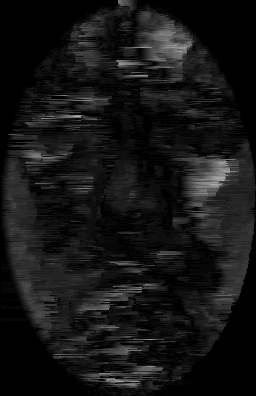
\includegraphics[trim = -1mm -1mm -1mm -1mm, width=0.12\textwidth]{classdb/A-norm-D} }
 \subfloat { \label{fig:row1-3} 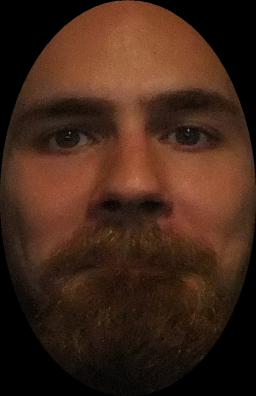
\includegraphics[trim = -1mm -1mm -1mm -1mm, width=0.12\textwidth]{classdb/B-norm} }
 \subfloat { \label{fig:row1-4} 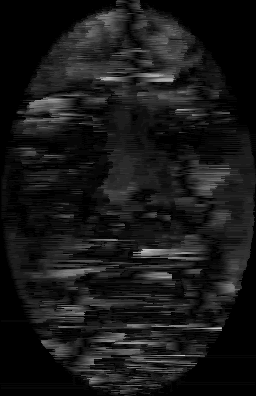
\includegraphics[trim = -1mm -1mm -1mm -1mm, width=0.12\textwidth]{classdb/B-norm-D} }\\

\begin{center}
\line(1,0){300}
\end{center}

 \subfloat { \label{fig:row2-1} 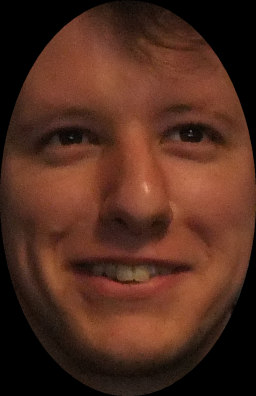
\includegraphics[trim = -1mm -1mm -1mm -1mm, width=0.12\textwidth]{classdb/C-norm} }
 \subfloat { \label{fig:row2-2} 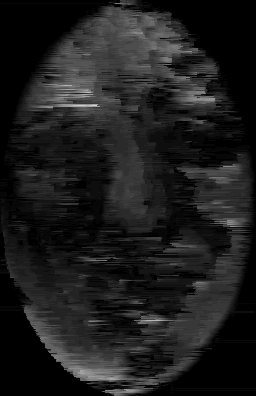
\includegraphics[trim = -1mm -1mm -1mm -1mm, width=0.12\textwidth]{classdb/C-norm-D} }
 \subfloat { \label{fig:row2-3} 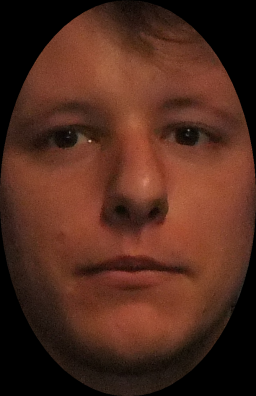
\includegraphics[trim = -1mm -1mm -1mm -1mm, width=0.12\textwidth]{classdb/D-norm} }
 \subfloat { \label{fig:row2-4} 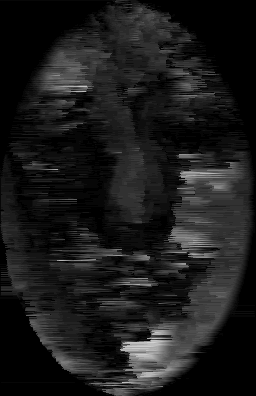
\includegraphics[trim = -1mm -1mm -1mm -1mm, width=0.12\textwidth]{classdb/D-norm-D} }\\

\begin{center}
\line(1,0){300}
\end{center}

 \subfloat { \label{fig:row3-1} 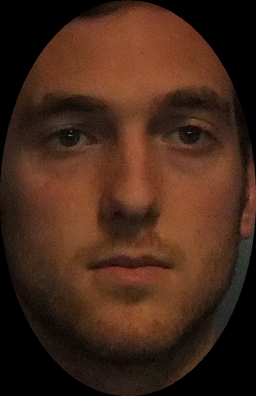
\includegraphics[trim = -1mm -1mm -1mm -1mm, width=0.12\textwidth]{classdb/E-norm} }
 \subfloat { \label{fig:row3-2} 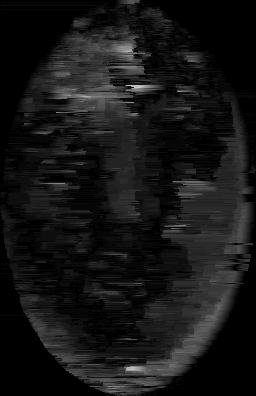
\includegraphics[trim = -1mm -1mm -1mm -1mm, width=0.12\textwidth]{classdb/E-norm-D} }
 \subfloat { \label{fig:row3-3} 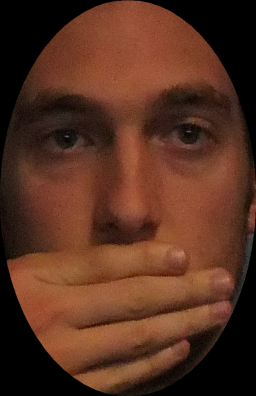
\includegraphics[trim = -1mm -1mm -1mm -1mm, width=0.12\textwidth]{classdb/F-norm} }
 \subfloat { \label{fig:row3-4} 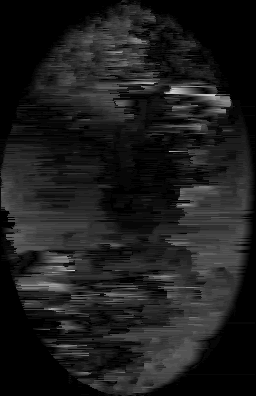
\includegraphics[trim = -1mm -1mm -1mm -1mm, width=0.12\textwidth]{classdb/F-norm-D} }\\

\begin{center}
\line(1,0){300}
\end{center}

 \subfloat { \label{fig:row4-1} 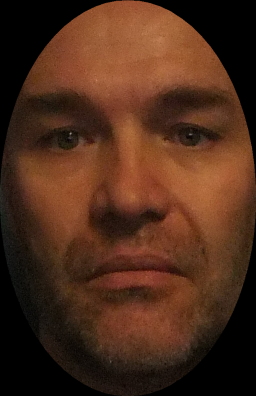
\includegraphics[trim = -1mm -1mm -1mm -1mm, width=0.12\textwidth]{classdb/G-norm} }
 \subfloat { \label{fig:row4-2} 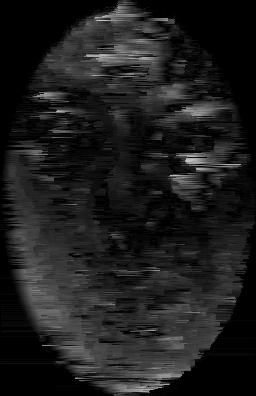
\includegraphics[trim = -1mm -1mm -1mm -1mm, width=0.12\textwidth]{classdb/G-norm-D} }
 \subfloat { \label{fig:row4-3} 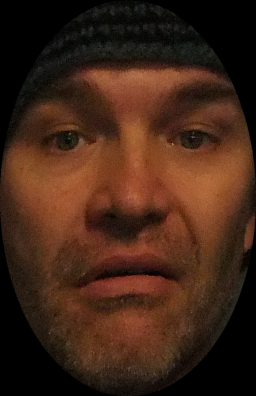
\includegraphics[trim = -1mm -1mm -1mm -1mm, width=0.12\textwidth]{classdb/H-norm} }
 \subfloat { \label{fig:row4-4} 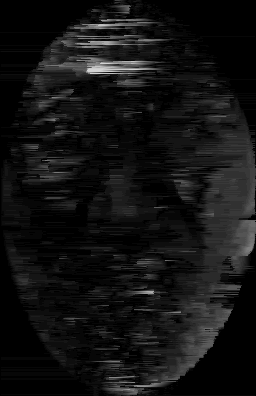
\includegraphics[trim = -1mm -1mm -1mm -1mm, width=0.12\textwidth]{classdb/H-norm-D} }\\

\begin{center}
\line(1,0){300}
\end{center}

 \caption[A sample of our PCA database]{A sample of images from our PCA database. Each row of images
describes two images from a class, alongside their associated depth map. These are the rectified,
registered $256\times396$ resolution images taken with the W3 camera.}
 \label{fig:classdb}
\end{figure}





